% ============================================================
%  Conceptual Topography
%  A Field-Theoretic Account of Conceptual Landscapes
%
%  Author : Yuhki Endoh (Independent Researcher)
%  Repo   : conceptual-topography/
%  Series : VED × IFGT Application Layer 1
%  Date   : 2026
% ============================================================

\documentclass[11pt, a4paper]{article}

% ---- packages ----
\usepackage{amsmath, amssymb, amsthm}
\usepackage{geometry}
\usepackage{hyperref}
\usepackage{graphicx}
\usepackage{caption}
\usepackage{booktabs}
\usepackage{longtable}
\usepackage{array}
\usepackage{xcolor}
\usepackage{cleveref}
\usepackage{microtype}
\usepackage{natbib}

\geometry{
  top=25mm, bottom=25mm,
  left=25mm, right=25mm
}

% ---- fonts ----
\usepackage{palatino}
\usepackage[T1]{fontenc}

% ---- colors ----
\definecolor{vedblue}{RGB}{30,100,180}
\definecolor{ifgtorange}{RGB}{180,80,20}
\definecolor{clgreen}{RGB}{40,140,80}

% ---- theorem environments ----
\newtheorem{definition}{Definition}[section]
\newtheorem{proposition}{Proposition}[section]
\newtheorem{remark}{Remark}[section]

% ---- notation macros (Master Table v2.1) ----
\newcommand{\JI}{J_{\!I}}
\newcommand{\JC}{J_{\!C}}
\newcommand{\Cmax}{C_{\max}}
\newcommand{\Phistar}{\Phi^{*}}
\newcommand{\seddto}{\xrightarrow{\;\mathrm{sed.}\;}}

% ---- hyperref setup ----
\hypersetup{
  colorlinks = true,
  linkcolor  = vedblue,
  citecolor  = clgreen,
  urlcolor   = ifgtorange,
  pdftitle   = {Conceptual Topography},
  pdfauthor  = {Yuhki Endoh},
}

% ============================================================
\begin{document}
% ============================================================

% ---- title ----
\title{%
  \textbf{Conceptual Topography}\\[6pt]
  {\large A Field-Theoretic Account of Conceptual Landscapes}\\[4pt]
  {\normalsize VED $\times$ IFGT Application Layer 1}
}
\author{%
  Yuhki Endoh\\
  {\small Independent Researcher}
}
\date{2026}
\maketitle

% ---- scope declaration (Master Table v2.1) ----
\begin{quote}
\small\itshape
This paper uses the VED$\times$IFGT framework described in
\cite{VED_vol1,VED_vol2,VED_vol3,VED_vol4,IFGT} as a source of formal vocabulary.
Its notation was attributed to the Master Variable Table v2.1; the exact
artifact and version behind that attribution remain unresolved.
The present work does not redefine $C$, $I$, $\Phi$, $\JI$, $\JC$, $\sigma$,
or $\tau$; it proposes cognitive uses of this vocabulary without claiming a
typed derivation from the upstream theories.
The primary definition $\Phi = K*I$ is used throughout;
the linear approximation $\Phi \approx -\alpha C + \Phi_0$ is employed only where
explicitly stated.
Semantic, psychological, or intentional interpretations of these quantities
are not assumed unless explicitly stated.
The strict inequality $C < \Cmax$ is retained as a model constraint.
Conceptual-domain uses of $I$, $C$, and $\Phi$ are proposed projected
or coarse-grained interpretations within a cognitive observation window.
Shared notation does not establish shared quantities or a typed translation.
Formal conditions, including the scope of the force relation, positivity
preservation, token-coupling signatures, and the long-time limit, remain
unresolved where not specified.

The definitions below fix local model vocabulary. Semantic and cognitive
readings are interpretations; phenomenal readings are proposed correspondences,
not explanations of subjective experience. The paper supplies neither
operational mappings nor model-linked empirical validation. The existing
figures and their captions are scoped as conceptual schematics, not measured
trajectories, executed dynamics, or evidence for the proposed interpretations.
\end{quote}

\vspace{4pt}

% ---- sections ----
% ============================================================
%  Abstract
% ============================================================

\begin{abstract}
This paper presents Conceptual Topography (CT), a field-theoretic
account of conceptual landscapes, as the first application layer of
the VED$\times$IFGT framework.
Conceptual landscape is a model-local designation for the proposed
long-time geometry of the information potential field $\Phi(x,\tau)$
under recursive token--field interaction. Sedimentation, its relation to
thought, and the invisible-terrain picture are interpretations, not
established convergence or phenomenal-access results.

Within the VED$\times$IFGT framework, CT organizes a proposal around
three coupled processes.
First, the continuous information field $I(x,\tau)$ is used in a proposed
cognitive-window interpretation of the VED$\times$IFGT relation
$I=f(1-C)$, with effective potential $\Phi = K * I$ providing the
geometry used to represent passability.
Second, discrete language tokens
$\ell_i = \mathcal{Q}[I,\Phi,C;\,\text{constraints}]$ act as
re-addressable discrete units assigned a local interaction with $\nabla\Phi$;
well deepening through reuse is a qualitative mechanism hypothesis.
Third, the recursive loop
$\Delta \to C \to I \to \Phi \to \JI \to \Delta$
describes a proposed feedback architecture. The sedimentation expression
$\Phi \seddto \Phistar$ is retained as a long-time template, with its
convergence and history-dependent interpretation unresolved.

The local structural definitions are retained: a concept is a locally
stable region of $\Phi$ satisfying $\nabla\Phi(x) \approx 0$; understanding
is a temporary reduction in traversal cost across such a region.
Thought is a proposed cognitive reading of trajectories associated with
the formal flow field $\JI$, not identical to that field.
Within the model, strict positivity $I(x,\tau) > 0$ is interpreted as
excluding ordinary complete conceptual closure. Further differentiation
is proposed under residual asymmetry, boundary structure, or new
perturbations, not guaranteed by positivity alone.

At the social scale, CT compares token functions and dominant costs.
Shared terrain, institutional attractors, and collective maintenance are
proposed social interpretations; identical individual/collective dynamics
and institutional explanations are not established.

This work does not redefine any variable of the VED$\times$IFGT framework;
it proposes cognitive and linguistic uses of that vocabulary without
establishing typed inheritance, operational mappings, or empirical validation.
\end{abstract}

\newpage
\tableofcontents
\newpage

% ============================================================
%  §1  Introduction
% ============================================================

\section{Introduction}
\label{sec:introduction}

% ---- scope declaration ----
This paper operates within the VED$\times$IFGT framework
\citep{VED_vol1, IFGT} and proposes model-local interpretations in the
domain of conceptual structure and thought dynamics.
The intended notation continuity with the Master Variable Table v2.1 is
retained, while its exact source/version and typed inheritance remain unresolved.
The framework developed here is called Conceptual Topography (CT);
the phrase ``conceptual terrain'' refers to the same object when the
intuitive metaphor is emphasized.

% ---- motivation ----
\subsection{The Problem of Conceptual Structure}

What is a concept?
The standard answer places concepts in the semantic domain:
a concept is a meaning-bearing unit, a mental representation,
or a node in a propositional network.
This answer, while useful for many purposes, leaves the
\emph{dynamical} question unanswered.
How does a concept form, stabilize, and constrain subsequent thought?
How does understanding arise, and why does it sometimes fail to transfer
even when the relevant definitions are available?

The present paper approaches these questions from a different direction.
Rather than asking what a concept \emph{means}, we ask what structural
conditions allow a region of the information field to persist, be
re-entered at low cost, and systematically bias future dynamics.
This reframing shifts the problem from semantics to geometry.

% ---- position ----
\subsection{Position in the \texorpdfstring{VED$\times$IFGT}{VED x IFGT} Series}

The VED$\times$IFGT framework consists of two foundational layers.
Vortical Enclosure Dynamics (VED) describes the generation of structure
from difference, gradient, flow, and closure \citep{VED_vol1}.
Information Field Geometry Theory (IFGT) describes the complementary
informational structure that persists as quasi-closure in the region
where $C$ does not reach unity \citep{IFGT}.

The present work is positioned as \emph{Application Layer 1} of this
framework: it proposes cognitive and social interpretations of
IFGT's field-theoretic vocabulary.
It does not introduce new foundational variables; the VED$\times$IFGT
equation motivates candidate structural classes for organizing cognitive
phenomena, not an established existence or classification theorem.

The series architecture is:
\begin{center}
\begin{tabular}{ll}
\toprule
Layer & Theory \\
\midrule
L0 (generation) & VED \\
L0 (structure)  & IFGT \\
L1 (application) & \textbf{Conceptual Topography [this paper]} \\
L1 (application) & Consciousness Theory [repository companion] \\
L1 (application) & Intelligence Theory [repository companions] \\
\bottomrule
\end{tabular}
\end{center}

% ---- main claims ----
\subsection{Main Claims}

The paper retains local definitions and proposes the following interpretations.
Definitions of concept and understanding do not establish the cognitive or
phenomenal correspondences discussed alongside them:

\begin{enumerate}
  \item A \textbf{concept} is a locally stable region of the information
        potential $\Phi(x,\tau)$, defined by $\nabla\Phi(x)\approx 0$
        with stability under small perturbations.

  \item \textbf{Understanding} is a temporary reduction in traversal cost
        across a conceptual region, not the acquisition of correct meaning.

  \item \textbf{Thought} is interpreted using trajectories associated with
        the formal information flow $\JI$. This description includes bias
        from $\nabla\Phi$, not a complete path specified by the gradient
        alone, and does not require a directing subject within the model.

  \item \textbf{Language tokens} are modeled as discrete re-addressable units
        that couple locally to $\nabla\Phi$ without carrying semantic
        content. Deepening through reuse is a hypothesis, with typing
        and update consequences still unresolved.

  \item Within the model, strict positivity $I(x,\tau)>0$ is interpreted
        as excluding ordinary complete conceptual closure. Further
        differentiation is a conditional proposal, compatible with local
        quiescence and not implied pointwise by positivity alone.

  \item At the \textbf{social scale}, a comparison of token roles motivates
        proposed shared terrain, institutional attractor analogies, and
        a local collective-maintenance description. A common dynamics or
        general definition of intelligence is not established.
\end{enumerate}

% ---- structure of the paper ----
\subsection{Structure of the Paper}

Section~\ref{sec:intuitive} presents an intuitive picture of conceptual
landscapes.
Section~\ref{sec:formal} proposes correspondences from VED$\times$IFGT
vocabulary to conceptual phenomena.
Section~\ref{sec:core} presents the existing field and coupling expressions
with their local definitions and unresolved formal scope.
Section~\ref{sec:structural} organizes candidate structural classes.
Section~\ref{sec:dynamics} develops qualitative hypotheses of sedimentation,
forgetting, and conceptual change.
Section~\ref{sec:multiscale} treats the scale inversion from individual
to social landscapes.
Section~\ref{sec:pathologies} describes proposed failure regimes and limits.
Section~\ref{sec:note} connects the formal structure to the intuitive
recorded note vocabulary, while preserving unresolved artifact attribution.
Section~\ref{sec:discussion} discusses implications and open questions.
Section~\ref{sec:conclusion} concludes.

% ============================================================
%  §2  Intuitive Picture
% ============================================================

\section{Intuitive Picture}
\label{sec:intuitive}

Before introducing the formal apparatus, we sketch the intuitive picture
that motivates the technical development.

\subsection{Thought as Movement Across Terrain}

Consider the experience of working through a difficult problem.
Some directions of thought feel natural and low-cost; others require
effort and tend to be abandoned.
Some ideas return repeatedly without deliberate intention; others, once
visited, leave no trace.
We propose to interpret the sense of understanding in terms of a change
in the ease of moving through a region of thought, rather than as the
acquisition of a new object. This phenomenological correspondence is
separate from the model's threshold definition of understanding.

These experiential examples motivate a spatial metaphor: thought moves across a
terrain whose shape is not fixed in advance but is formed by the
history of prior movement.
In this proposed picture, frequently traversed paths become smoother,
while less visited regions become less accessible.
The invisible terrain is a metaphor for experiencing ease or difficulty
without inspecting the proposed geometry, not a claim of proven inaccessibility.

This is the intuitive core of Conceptual Topography.
Figure~\ref{fig:potential-geometry} summarizes this geometric picture.

\begin{figure}[t]
  \centering
  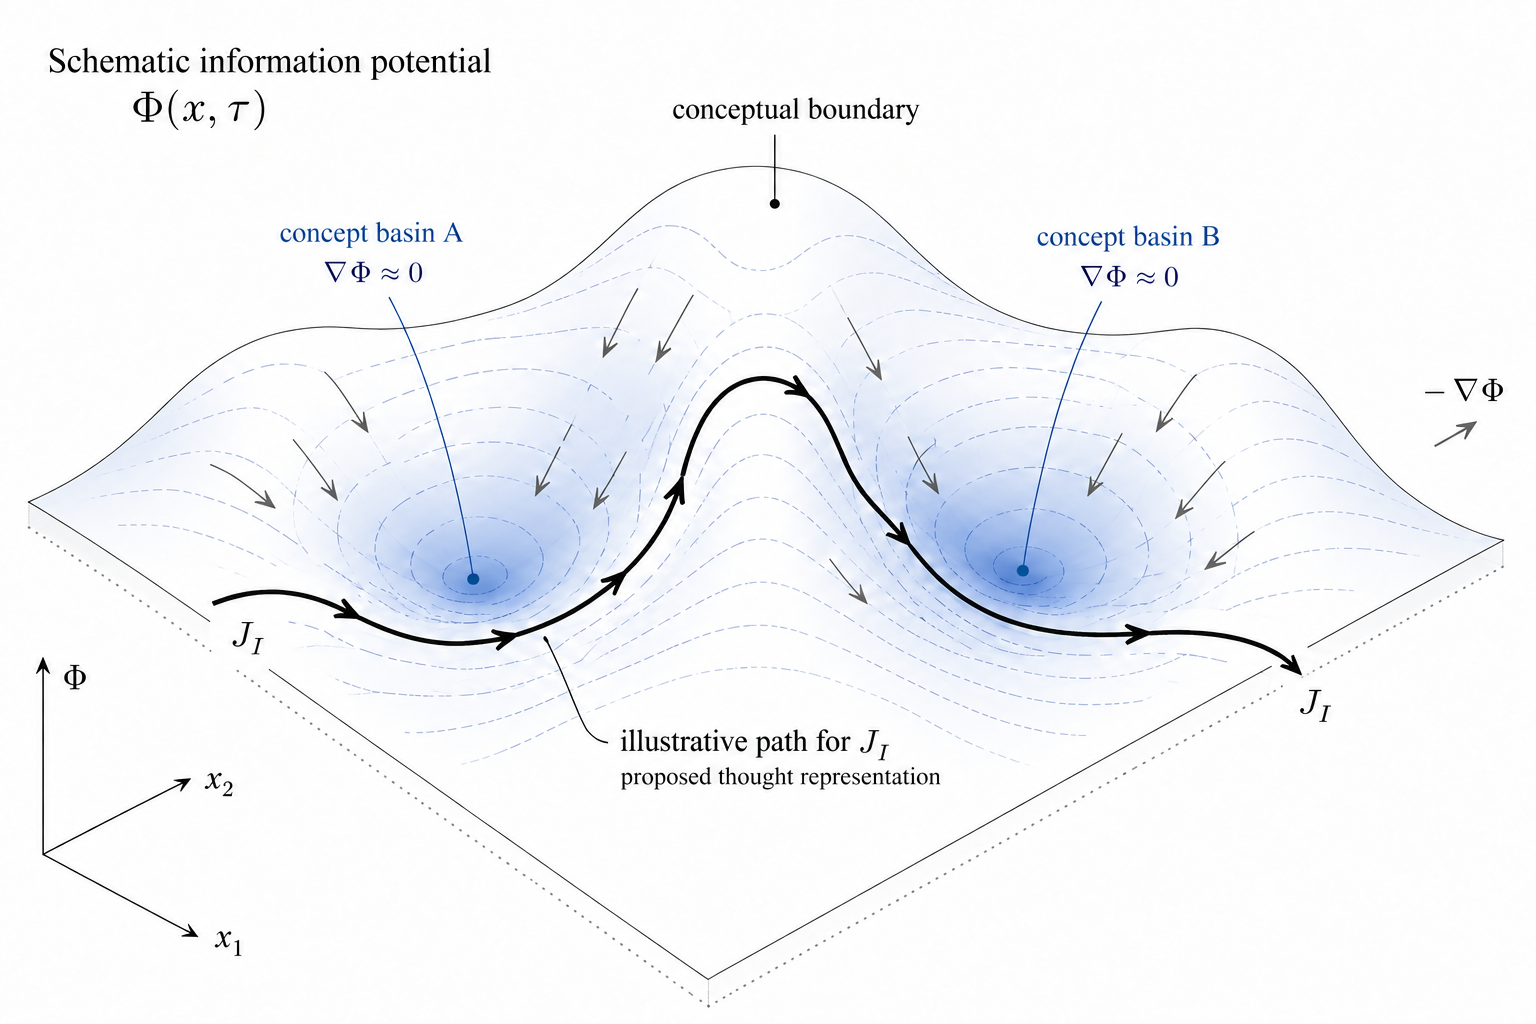
\includegraphics[width=0.92\linewidth]{figures/fig1_potential_geometry.png}
  \caption{
  Schematic conceptual landscape as information-potential geometry.
  The surface illustrates the model potential $\Phi(x,\tau)$.
  Basins depict the local concept definition where $\nabla\Phi \approx 0$.
  The drawn path is an illustrative representation associated with the flow field $J_I$, not the field itself or a measured thought path.
  Its cognitive reading is proposed; ridges illustrate model-level conceptual boundaries.
  }
  \label{fig:potential-geometry}
\end{figure}

The terrain is the model-local reading of the information potential
$\Phi(x,\tau)$ as history-shaped geometry associated with information flow
$\JI$. Movement is a trajectory representation associated with
$\JI$, with $-\nabla\Phi$ contributing a directional bias rather than
specifying the entire path. Calling this movement thought is a further
cognitive interpretation, not a field/path/content identity.
The understanding picture uses a local reduction in $|\nabla\Phi|$
in a previously difficult region. Its correspondence to felt ease remains
a hypothesis: the formal threshold definition is not independent evidence
for a sense of understanding.

\subsection{Concepts as Valleys}

In this picture, a concept is a valley in the potential landscape:
a region of low $\Phi$ toward which trajectories are naturally drawn.
Valley depth is proposed to reflect repeated traversal, and width is
compared with the range of contexts in which a concept applies. These
comparisons do not supply independent semantic measurements.

Crucially, the valley does not contain a meaning.
It is described as a \emph{dynamical attractor}: a region that biases
subsequent trajectories in the model, with patterns of thought as the
proposed cognitive interpretation.
What we call the ``meaning'' of a concept is, in this framework,
the set of trajectories that the attractor makes available.

\subsection{Linguistic Tokens as Terrain-Shaping Operations}

Linguistic tokens --- understood broadly to include not only natural
language words but any discrete, re-addressable medium capable of acting
on the field as a localized perturbation: symbols, emblems, gestures,
diagrams, mathematical notation, and so on --- are not assigned intrinsic
meanings in this account.
They are modeled as localized perturbations that bias the landscape.
Repeated use in similar contexts is hypothesized to deepen an associated
valley, while declining reuse is associated with shallowing.
More similar sender and receiver landscapes are proposed to support more
similar responses to a perturbation; divergence may contribute to
communication failure. This comparative hypothesis neither exhausts the
explanation of communication nor estimates geometry from communication
success.

\subsection{The Invisible GPU}

The invisible-GPU metaphor proposes a structural interpretation of
cognition without direct inspection of the landscape.
It is used to organize experiential examples: thoughts coming naturally,
connections suggesting themselves, and understanding arriving suddenly
rather than being constructed step by step.

These experiences are proposed to correspond to the geometry of $\Phi$,
rather than to intrinsic meanings stored in that geometry.
This is not an explanation of how subjective experience is generated.

The following sections distinguish this intuitive vocabulary from the
formal definitions and the unresolved cognitive and phenomenal mappings.

% ============================================================
%  §3  Formal Mapping
% ============================================================

\section{Formal Mapping}
\label{sec:formal}

This section records proposed correspondences between VED$\times$IFGT
variables and conceptual phenomena. The table separates formal roles from
model-local interpretations; it does not supply operational mappings.
The attribution to the Master Variable Table v2.1 remains subject to the
source-provenance limitation stated at the beginning of the paper.

\subsection{The Background Field}

The information density field $I(x,\tau) = f(1-C(x,\tau))$ is used as
the continuous field in the model of conceptual structure.
In this paper, $I$ is not a new cognitive primitive but a proposed
cognitive-window interpretation of the IFGT information-density vocabulary,
not an established typed identity.
In this local interpretation, $I$ represents the density of unresolved
informational tension at position $x$ and evolution parameter $\tau$:
regions described as quasi-closed, neither fully stabilized nor fully
dissipated.

High $I$ is proposed to correspond to conceptually active regions; low $I$
to regions where structure has largely closed. This is not a calibrated
activity measure.
Within this account, the strict positivity $I(x,\tau)>0$ is interpreted
as excluding complete closure as an ordinary conceptual state.
It does not by itself guarantee a nonzero local gradient or flow.
The role of residual asymmetry, nonuniform history, and boundary structure
in gradient formation remains a model-level hypothesis.

The information potential
\begin{equation}
  \Phi(x,\tau) = (K * I)(x,\tau)
  \label{eq:Phi_primary}
\end{equation}
is the primary geometric object.
Its landscape reading is a model-level interpretation of accumulated bias.
The potential gradient contributes an effective directional bias; it does
not alone determine a complete trajectory, since the flow relation also
contains a diffusion term. The field-to-trajectory-to-thought correspondence
is not supplied as a typed or operational map.

\subsection{Variable Correspondence Table}

\begin{center}
\renewcommand{\arraystretch}{1.5}
\begin{tabular}{p{0.22\textwidth}p{0.48\textwidth}p{0.22\textwidth}}
\toprule
\textbf{VED$\times$IFGT variable} &
\textbf{Conceptual domain interpretation} &
\textbf{Formal role} \\
\midrule
$C(x,\tau)$ &
Degree of conceptual fixation at $x$ &
Background field; $C \in [0,\Cmax)$ \\
$I(x,\tau) = f(1-C)$ &
Density of unresolved conceptual tension &
Central field; $I > 0$ always \\
$\Phi = K*I$ &
Model-local conceptual landscape &
Potential geometry \\
$\nabla\Phi$ &
Proposed bias toward lower cognitive resistance &
Constraint force on $\JI$ \\
$\JI = -D\nabla I + \mu F_I$ &
Proposed representation of thought &
Formal flow field \\
$\sigma = \sigma_d - \sigma_p - \sigma_b$ &
Rate of landscape deformation &
Source term \\
$\Delta$ &
Novel experience, perception, or linguistic input &
Driving source \\
$\delta I$ &
Unresolved conceptual residue &
Trace that constitutes $I$ \\
$\tau$ &
Proposed experiential-time correspondence &
Formal evolution / ordering parameter \\
$\ell_i = \mathcal{Q}[I,\Phi,C;\cdot]$ &
Reusable linguistic token (natural language word, symbol, emblem,
gesture, diagram, formula, or any discrete unit capable of acting on the
field as a localized perturbation) &
Proposed action on $\Phi$; signature unresolved \\
$\Phistar$ &
Mature, sedimented conceptual landscape &
Long-time attractor of $\Phi$ \\
$\Cmax$ &
Ideal complete-closure boundary &
Boundary representation, not an ordinary state \\
\bottomrule
\end{tabular}
\end{center}

The temporal parameter orders formal evolution; its experiential reading
is a separate proposal, not a clock calibration. Likewise, the sedimented
landscape and long-time-attractor labels retain the unresolved limit and
history-dependent interpretation discussed in Section~\ref{sec:core}.

\begin{remark}[Notational remark]
The operator $\mathcal{Q}$ is called a quantization operator because its
action --- extracting discrete, re-addressable units from a continuous
field configuration --- is compared structurally with the passage from
continuous variables to discrete values. This is an informal analogy,
not a mathematical isomorphism or a shared physical operation.
The term ``quantum'' is not used as a theoretical claim within CT, but
the analogy is preserved in the name of this operator.
\end{remark}

\subsection{What the Mapping Does Not Claim}

The proposed correspondences above do not introduce semantic content,
intentionality, or psychological states into the formalism.
In particular:
\begin{itemize}
  \item $\Phi$ is not a meaning field. It is a dynamical constraint
        geometry used to describe relative transition costs within the model.
  \item $\JI$ is not thought content. It is the formal flow field; a trajectory
        description and its interpretation as thought are distinct uses.
        Content appearing in experience is treated as a downstream topic,
        not a consequence established by identifying these uses.
  \item $\ell_i$ is not a meaning unit. It is a discrete re-addressable
        unit that couples locally to $\nabla\Phi$.
\end{itemize}
These exclusions are methodological necessities, not claims about the
ultimate nature of meaning or experience.

% ============================================================
%  §4  Core Equations
% ============================================================

\section{Core Equations}
\label{sec:core}

\paragraph{Formal scope and unresolved assumptions.}
The domain, geometry and measure, and parameter ranges are not fully
specified. Additional assumptions and conventions in related IFGT
formulations, including normalization choices, are not automatically
adopted as CT specialization conditions. The scope statements below
identify missing specifications; they do not supply them.

\subsection{Field Evolution}

The balance relation is used here as a model-level formal template.
A complete initial-boundary-value problem, including the domain,
initial and boundary conditions, regularity, and positivity-preservation
conditions, is not specified. Use of the relation does not establish
existence, uniqueness, or well-posedness:
\begin{equation}
  \frac{\partial I}{\partial\tau} + \nabla\cdot\JI = \sigma,
  \label{eq:I_evolution}
\end{equation}
where the information flow is
\begin{equation}
  \JI = -D\nabla I + \mu F_I, \qquad F_I = -\nabla\Phi = \alpha\nabla C,
  \label{eq:JI}
\end{equation}
In the force relation, the first equality defines the effective force
from the negative potential gradient. The subsequent closure-gradient
equality is intended as a local/effective specialization, not as a
derivation from the primary convolution, which remains the general
field relation. The approximation regime and the assumptions under
which that specialization is valid remain to be fixed.

The generation term decomposes as
\begin{equation}
  \sigma = \sigma_{\mathrm{drive}} - \sigma_{\mathrm{dissip}} - \sigma_{\mathrm{barrier}}.
  \label{eq:sigma}
\end{equation}

The three contributions are:
\begin{align}
  \sigma_{\mathrm{drive}}  &= a\Delta\!\left(1 - \frac{C}{C_*}\right),
  \label{eq:sigma_drive}\\
  \sigma_{\mathrm{dissip}} &= \Gamma C,
  \label{eq:sigma_dissip}\\
  \sigma_{\mathrm{barrier}}&= \frac{\kappa_B}{\Cmax - C}.
  \label{eq:sigma_barrier}
\end{align}

Here $C_*$ denotes the effective saturation scale of conceptual
quasi-closure within the observation window, while $\Cmax$ denotes the
ideal complete-closure boundary.
In general $C_* < \Cmax$ for conceptual regimes.

The following are effective cognitive interpretations, not measured mechanisms:
$\sigma_{\mathrm{drive}}$ represents the influx of novel input
(perception, linguistic perturbation, reward signal);
$\sigma_{\mathrm{dissip}}$ represents the natural decay of
unresolved tension (forgetting, habituation);
$\sigma_{\mathrm{barrier}}$ represents a projected or coarse-grained
effective resistance against conceptual overclosure.
It should not be read as a fundamental external prohibition; it is the
cognitive-domain analogue of the effective barrier notation used in
VED and IFGT.
The reciprocal form does not by itself prove dynamical inaccessibility
of the stated upper boundary. Divergence of a reciprocal expression and
invariance under the full evolution are distinct claims; neither endpoint
behavior nor invariant-domain conditions are established here.

\subsection{Token--Field Coupling}

The present architecture treats discrete, re-addressable structures as
a proposed requirement for stable, low-cost recursion. The motivation is
that revisiting a continuous field configuration may be costly and
drift-prone; this is not a general impossibility claim about continuous
systems. Re-addressability is intended to support reuse of complex states.
Figure~\ref{fig:token-field-coupling} illustrates the coupling hypothesis,
not an executed demonstration of its consequences.

\begin{figure}[t]
  \centering
  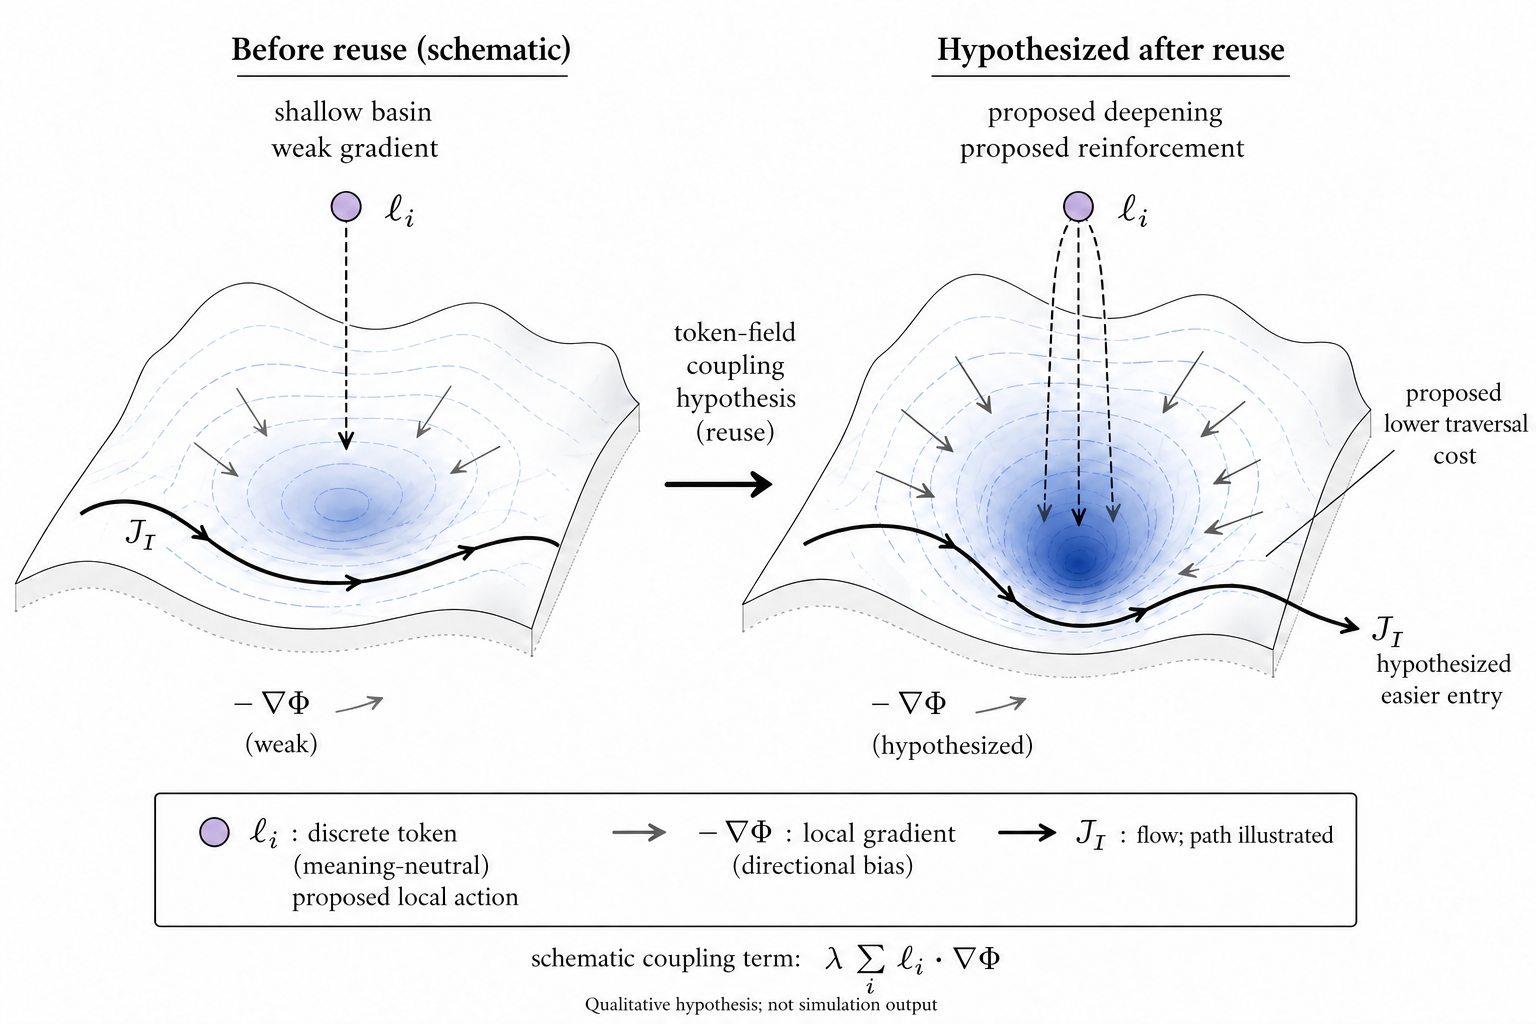
\includegraphics[width=0.95\linewidth]{figures/fig2_token_field_coupling.png}
  \caption{
  Schematic token--field coupling hypothesis, not simulation output.
  Discrete tokens $\ell_i$ are not assigned intrinsic meaning; their proposed local coupling to $\nabla\Phi$ motivates the illustration.
  Deepening and lower traversal cost for paths associated with $J_I$ are hypothesized effects, not executed or derived results.
  The expression $\lambda \sum_i \ell_i \cdot \nabla\Phi$ remains schematic: token realization and pairing are unresolved.
  }
  \label{fig:token-field-coupling}
\end{figure}

The medium that enables this structure is the linguistic field, where
``linguistic'' is understood broadly to include not only natural language
but any discrete, re-addressable medium capable of acting on the field
as a localized perturbation: symbols, emblems, gestures, diagrams,
mathematical notation, and so on.

Linguistic tokens $\ell_i$ (discrete units drawn from any such medium)
are assigned the following effective token--field coupling expression:
\begin{equation}
  \mathcal{L}_{\mathrm{eff}} = \mathcal{L}_{\mathrm{field}}[I]
  + \mathcal{L}_{\mathrm{token}}[\ell]
  + \lambda \sum_i \ell_i \cdot \nabla\Phi.
  \label{eq:coupling}
\end{equation}

The proposed coupling role is dynamical rather than semantic: tokens do
not encode meanings but are hypothesized to bias the local evolution of
$\Phi$ through repeated interaction.
Gradient reinforcement and well deepening are qualitative mechanism
hypotheses, not consequences established merely by writing the term.
The coupling expression remains schematic with respect to the numerical
or vector realization of discrete tokens and the pairing implied by the
dot notation: neither is formally specified. The mathematical kind of
the effective, field, and token Lagrangian terms, and the coupling-parameter
specification, also remain unresolved. No Euler--Lagrange or other
variational or update dynamics are derived from this expression here.

\subsection{Sedimentation and Conceptual Landscape Formation}

The long-time expression below is retained as a sedimentation template
for repeated token--field interaction, not as an established convergence
result. Figure~\ref{fig:minimal-recursive-loop} summarizes the proposed
feedback architecture with the framework's irreversible-ordering premise.

\begin{figure}[t]
  \centering
  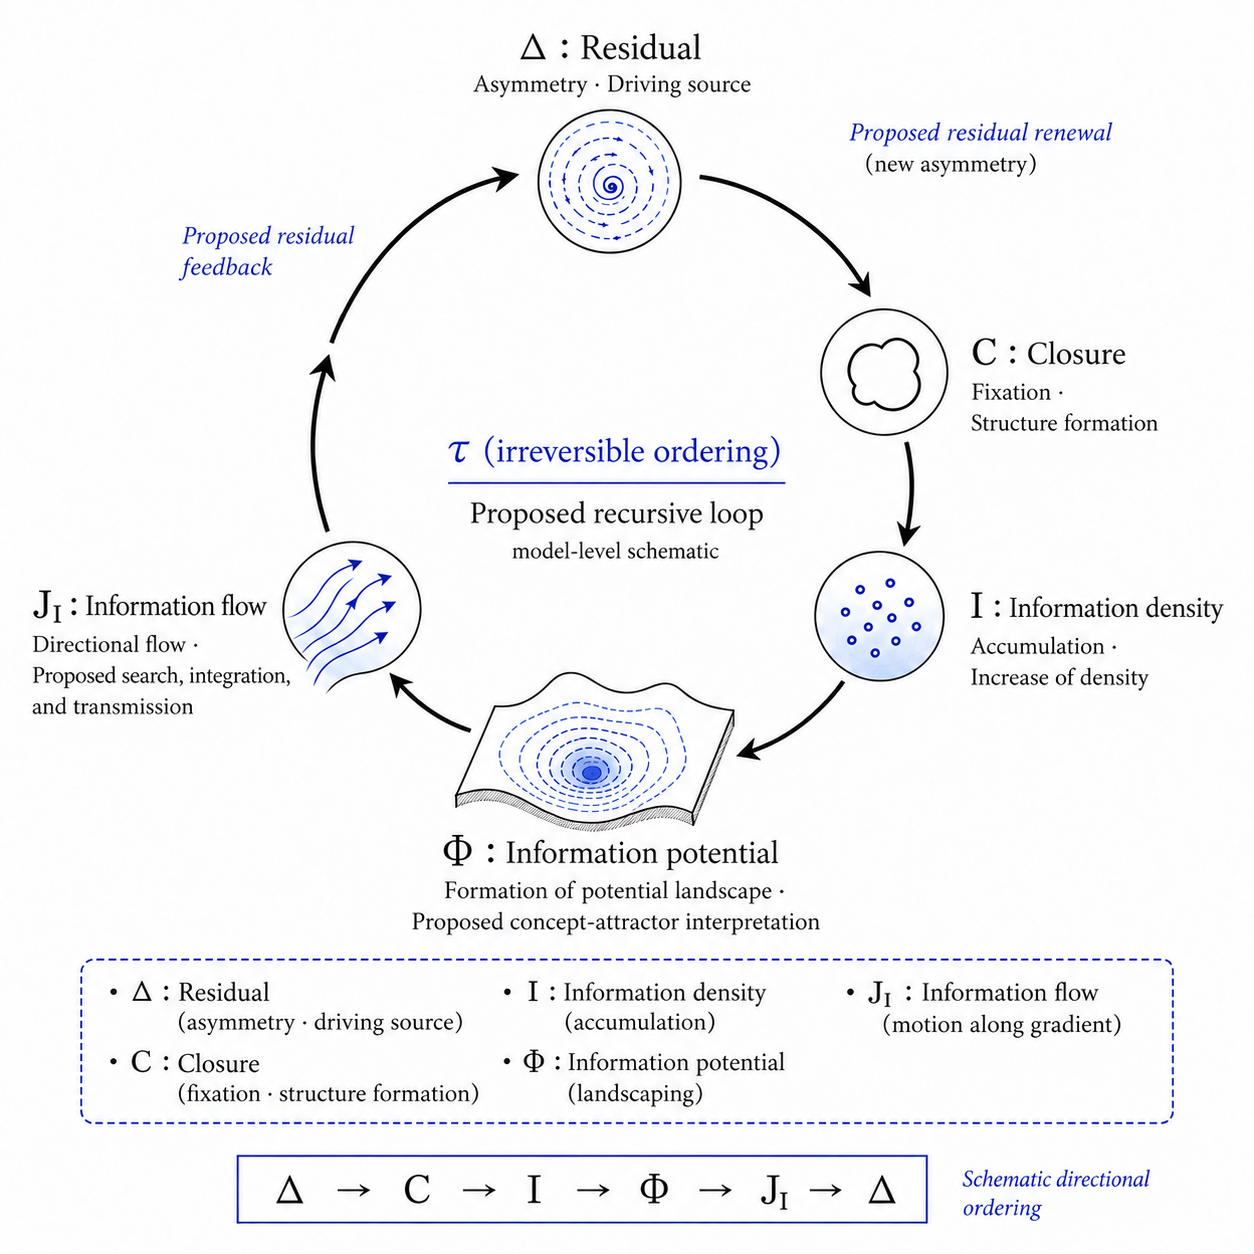
\includegraphics[width=0.82\linewidth]{figures/fig3_minimal_recursive_loop.png}
  \caption{
  Proposed recursive loop in the VED$\times$IFGT vocabulary.
  The schematic sequence
  $\Delta \to C \to I \to \Phi \to J_I \to \Delta$
  links residual asymmetry $\Delta$, closure $C$, information density $I$, potential structure $\Phi$, and information flow $J_I$ within the proposed feedback architecture.
  The ordering parameter $\tau$ expresses the model's irreversible-ordering premise; arrows are not a proof of causality or an executed dynamical witness.
  }
  \label{fig:minimal-recursive-loop}
\end{figure}

\begin{equation}
  \Phi(x,\tau) \;\xrightarrow{\;\tau\to\infty\;}\; \Phistar(x).
  \label{eq:sedimentation}
\end{equation}

The arrow is a long-time template with no specified convergence mode.
The following history interpretation retains unresolved formal and
source-version status: how the displayed limit target relates to continued
reshaping under renewed input is not decided here. The nonuniqueness and
nonstatic wording below is version-sensitive; no interpretation is selected
to settle that difference.

$\Phistar$ is the sedimented conceptual landscape.
It is not necessarily unique or static; it reflects the history of
all prior interactions and continues to be reshaped by new input,
though at decreasing rate as the landscape matures.

\subsection{Concept Definition}

\begin{definition}[Concept]
A \emph{concept} at position $x$ is a locally stable region of the
information potential satisfying:
\begin{equation}
  \nabla\Phi(x) \approx 0, \qquad
  \text{with stability under small perturbations of } \JI.
  \label{eq:concept}
\end{equation}
The depth of the potential well at $x$ is proposed as a structural
correspondence for resistance to deformation; width is compared with
contextual range. These interpretations are not semantic calibrations.
\end{definition}

\begin{definition}[Understanding]
\emph{Understanding} a conceptual region $\mathcal{R}$ is the state
in which the traversal cost of $\JI$ through $\mathcal{R}$ has been
reduced to below a system-dependent threshold $\theta$:
\begin{equation}
  \int_{\mathcal{R}} |\nabla\Phi|\,dx < \theta.
  \label{eq:understanding}
\end{equation}
Here $\theta$ is a system-dependent effective threshold expressing the
allowable range of recursive cost.
Its concrete value depends on the structure of the system, including
$D$, $\mu$, $\alpha$, and related parameters, and is not specified in
the present work.
Understanding is not a binary state but a dynamical condition that can
be entered and exited as $\Phi$ evolves.
\end{definition}

The definition specifies a local model state, not an independent cognitive
or phenomenal criterion. Its proposed relation to felt ease must therefore
be assessed separately; defining a low-cost state does not explain the
experience of understanding.

\subsection{The Strict Positivity Constraint}

The strict-positivity statement is retained as a model-level admissibility
condition. This positive-range constraint, the positive-output premise
below, and preservation under the full balance evolution are separate
formal burdens; their justification is not established here. The statement,
\begin{equation}
  \boxed{I(x,\tau) > 0 \qquad \forall\,x,\,\tau,}
  \label{eq:positivity}
\end{equation}
is stated with $C < \Cmax$ and the positive-output premise $I = f(1-C) > 0$ for
$C < \Cmax$.
Here $\Cmax$ denotes the ideal complete-closure boundary, not an
ordinary attainable state of the conceptual system.

\begin{proposition}[No ordinary complete conceptual closure]
Within the VED$\times$IFGT model interpretation, $I>0$ excludes complete
conceptual closure as an ordinary dynamical state.
Separately, in nontrivial landscapes with residual asymmetry,
spatial inhomogeneity, or boundary structure, further gradients in $\Phi$
and available directions for $\JI$ are proposed to reappear.
This is a conditional differentiation hypothesis, not a consequence of
positivity alone. The closure interpretation is not the pointwise
mathematical claim that every positive $I$ must have
$\nabla\Phi\neq0$.
Without additional conditions, positivity alone does not imply nonzero
flow either; the full flow includes more than the potential-gradient
contribution.
\end{proposition}

\begin{remark}
This model-level distinction motivates a comparison with intelligence
and understanding, rather than deriving them from positivity.
Stable attractors may appear locally quiescent. Further differentiation
is proposed to remain possible under new perturbations or wider observation
windows; no unconditional learning or innovation guarantee is inferred.
\end{remark}

% ============================================================
%  §5  Structural Interpretation
% ============================================================

\section{Structural Interpretation}
\label{sec:structural}

\subsection{Candidate Structural Classes}

The VED$\times$IFGT framework motivates the following candidate
structural classes and cognitive interpretations.
The table organizes a model-based classification, not a formal existence
or classification theorem; detailed solution analysis and independent
cognitive correspondences remain future work.

\begin{center}
\renewcommand{\arraystretch}{1.5}
\begin{tabular}{p{0.29\textwidth}p{0.31\textwidth}p{0.30\textwidth}}
\toprule
\textbf{Candidate class} & \textbf{Field structure} & \textbf{Cognitive interpretation} \\
\midrule
Smooth gradient region   & $\nabla\Phi$ slowly varying     & Background cognitive disposition \\
Shallow metastable well  & $\nabla\Phi\approx 0$, small depth & Tentative or unstable concept \\
Deep stable well         & $\nabla\Phi\approx 0$, large depth & Entrenched concept or belief \\
Limit-cycle trajectory   & $\JI$ circulates without sedimentation & Recurring thought pattern \\
Barrier region           & $|\nabla\Phi|$ large             & Cognitive block or resistance \\
Ridge structure          & Local maximum of $\Phi$           & Conceptual boundary or category edge \\
\bottomrule
\end{tabular}
\end{center}

\subsection{Depth, Width, and Robustness}

Three geometric parameters characterize a conceptual attractor:

\textbf{Depth} ($-\min\Phi$ within the well) is proposed to correspond
to resistance to deformation by new input: deeper wells are compared with
more resistant concepts, shallower wells with more easily displaced ones.

\textbf{Width} (spatial extent of the sub-threshold region) is compared
with contextual range: broad wells with wider applicability, narrow wells
with more context-specific concepts.

\textbf{Robustness} (curvature of $\Phi$ at the minimum) is proposed
as a comparative indicator of precision: higher curvature is associated
qualitatively with sharper concepts, lower curvature with fuzzy or
polysemous ones. None of these semantic attributes is calibrated by
the geometric description alone.

These geometric attributes are not treated as fixed intrinsic properties;
they are modeled as evolving with $\Phi$ under the relations in
Eqs.~\eqref{eq:I_evolution}--\eqref{eq:sigma_barrier}.

\subsection{Conceptual Boundaries}

Ridge structures in $\Phi$ --- regions of locally high potential
separating neighboring wells --- represent conceptual boundaries in this
account: the distinctions between concepts.
These boundaries are not sharp lines but extended regions of high
traversal cost.

The qualitative hypothesis is that conceptual boundaries can shift under
repeated linguistic or experiential perturbation.
Tokens coupling near a ridge are proposed to reinforce it (deepening a
distinction) or erode it (merging adjacent concepts).
This is a candidate dynamical account of semantic drift and conceptual
change, not an established cognitive mechanism or semantic mapping.

\subsection{Vocabulary Selection and Distributional Description}

The full set of stabilized tokens $\{\ell_i\}$ is called a vocabulary
in this framework. The expression below selects a set by stability;
the broader description of vocabulary as distributed across the field
does not turn that set into a probability distribution:
\begin{equation}
  \mathcal{V} = \bigl\{\ell_i \;\big|\; S(\ell_i) > \epsilon \bigr\},
  \label{eq:vocabulary}
\end{equation}
where $S(\ell_i)$ is a stability functional intended to depend on reuse
frequency, persistence time, and basin depth, and $\epsilon$ is a
system-dependent threshold. The functional and threshold are not given
an extraction or calibration rule here.

Vocabulary is interpreted as a field-related organization reshaped by use.
Token frequency is proposed to relate to basin accessibility, not to serve
as a measure of semantic importance. Fuzzy, context-sensitive distinctions
are part of this interpretive picture, not an operational token criterion.

% ============================================================
%  §6  Dynamics
% ============================================================

\section{Dynamics}
\label{sec:dynamics}

\subsection{Sedimentation}

Sedimentation names the proposed process of well deepening and
conceptual stabilization under repeated token--field interaction.
The following three stages describe a functional feedback architecture,
not an executed dynamical witness. The first token/basin bootstrap and
the update consequences of coupling remain unresolved.

\textbf{Stage 1: Initial perturbation.}
In the proposed scenario, a novel input $\Delta$ is associated with
a $\sigma_{\mathrm{drive}}$ spike, a local increase in $I$, and a transient
potential gradient. The information flow $\JI$ is modeled as responding
to the perturbation; this is not a reconstructed thought path.

\textbf{Stage 2: Reinforcement.}
If the perturbation is repeated --- through subsequent exposure to
similar input or through internal recursive activation --- the local
gradient in $\Phi$ is hypothesized to be reinforced.
Well deepening is a proposed effect of token--field coupling
\eqref{eq:coupling}, not a result ensured by each reuse or by the
expression alone.

\textbf{Stage 3: Stabilization.}
The proposed stabilization stage associates well deepening with lower
traversal cost and subsequent reuse with further reinforcement.
A self-sustaining concept is the resulting maintenance hypothesis,
not a demonstrated consequence of the feedback architecture.

\subsection{Forgetting}

Forgetting is interpreted here by analogy with relaxation of $\Phi$
toward a flatter configuration when reuse frequency drops.
The existing dissipation term is retained as the formal template:
\begin{equation}
  \sigma_{\mathrm{dissip}} = \Gamma C.
\end{equation}
In this model picture, reduced accessibility is associated with a
redistribution of stability rather than erasure of stored symbols:
shallowing wells are proposed to raise traversal cost.
This does not establish that forgotten concepts never disappear.
Reactivation (remembering) is correspondingly modeled as re-deepening
through renewed token--field interaction, not identified with a universal
memory mechanism.

\subsection{Conceptual Change}

Conceptual change --- the shift in meaning, scope, or application of
an established concept --- is represented here using changes in
$\Phistar$: the merger of two wells, the splitting of one well into
two, or displacement within the landscape.
These geometric alternatives organize a proposed cognitive correspondence;
they do not resolve the long-time target or prove a topology-to-cognition map.

The candidate account associates such changes with sustained perturbation
relative to the depth of existing attractors, not with a calibrated
necessary or sufficient condition for belief revision.
The effective barrier term $\sigma_{\mathrm{barrier}}$ plays a
protective role in this effective description: as $C\to\Cmax$,
the resistance interpretation is compared with increasing difficulty
of changing a deeply entrenched concept.
This should be understood as an effective description of overclosure
within the conceptual observation window, not as an externally imposed
wall.
This offers a candidate account of resistance to belief revision;
the reciprocal term does not establish cognitive prohibition.

\subsection{Insight and the Rapid-Transition Hypothesis}

The sudden sense that a problem has been resolved or disparate ideas
connected motivates a proposed correspondence with rapid changes in the
local topology of $\Phi$.
Merging wells or a collapsing barrier provide a bifurcation-like
representation. A geometric transition, cognitive problem resolution,
and a felt event are distinct claims; no bifurcation theorem or
independent cognitive endpoint is supplied here.

The subjective sense of suddenness is hypothesized to correspond to
the threshold picture of accumulating perturbations followed by a rapid
transition. The picture does not independently identify perceptual
thresholds or explain felt suddenness merely by naming a transition.

% ============================================================
%  §7  Multi-scale / Multi-agent
% ============================================================

\section{Scale Inversion: Individual to Social}
\label{sec:multiscale}

\subsection{Comparing Functions and Dominant Costs}

The preceding model is interpreted at the level of an individual
cognitive system. In that interpretation, recursion and compression are
the proposed dominant costs: revisiting states and representing continuous
configurations with reusable discrete handles.
Language tokens are assigned an internal-control role under these
architectural assumptions.

A social extension is proposed by comparing this role with
synchronization and coordination among interacting agents.
Tokens are hypothesized to help stabilize shared trajectories and reduce
uncertainty about other agents' responses.
The table contrasts the proposed dominant costs and token functions;
it does not establish that individual and collective dynamics are identical:

\begin{center}
\begin{tabular}{lll}
\toprule
\textbf{Scale} & \textbf{Dominant cost} & \textbf{Token function} \\
\midrule
Individual & Recursion, compression & Internal control units \\
Social     & Synchronization, coordination & Shared landscape anchors \\
\bottomrule
\end{tabular}
\end{center}

The comparison proposes a similar re-addressing function under different
effective constraints. It does not establish unchanged token properties
across scales. Collective aggregation, a common state space, and a typed
translation remain unspecified; no shared-field measurement follows
from reusing the same notation.

\subsection{Social Conceptual Landscape}

The social hypothesis compares repeated exposure to shared linguistic
inputs, given sufficiently similar prior landscapes, with correlated
well deepening. Shared conceptual landscape is the model-level name
for this proposed organization.

In this picture, shared terrain is distributed across agents and
maintained through ongoing linguistic interaction, rather than stored
in one agent. History-shaped collective geometry is an interpretation
of those interactions, not a measured collective field.

\subsection{Norms, Institutions, and Paradigms}

Deeply sedimented social regions are compared structurally with norms,
institutions, and scientific paradigms.
This attractor analogy uses the collective $\Phi$ to represent persistence;
it is not an identity between institutions and formal attractors.

A separate hypothesis relates depth to stability and deviation cost,
and coordinated perturbation to institutional change. It offers a way
to consider persistence without making central enforcement the sole
explanation, not evidence that enforcement is unnecessary.
Historical difficulty of paradigm shifts is a possible comparison target,
not a result explained by well depth. Independent institutional criteria
and depth estimation remain unresolved; stability cannot serve as both
the definition of depth and independent evidence for its explanatory role.

\subsection{Intelligence as Landscape Maintenance}

Within this social-scale account, we use a local functional designation
for the proposed distributed process:
\begin{quote}
\itshape
Social intelligence, as used here, names distributed maintenance,
synchronization, and reshaping of conceptual landscapes through language.
\end{quote}

This naming is not an established general definition or generation of
intelligence, nor does it exclude individual intelligence. Its relation
to the repository's Intelligence theories is a conceptual handoff, not
validation transferred from downstream work.

Individual agents are modeled as transient participants in this process:
they traverse the landscape, introduce local deformations, and transmit
stabilized structures to subsequent agents through externalized
linguistic logs.

The strict positivity $I>0$ motivates an analogous nonclosure reading
for the proposed social landscape, not a derivation of collective dynamics.
Further differentiation and innovation are proposed possibilities under
new perturbations or wider observation windows that reactivate residual
asymmetries, not outcomes guaranteed by positivity alone.

% ============================================================
%  §8  Pathologies and Limits
% ============================================================

\section{Pathologies and Limits}
\label{sec:pathologies}

\subsection{Deliberate Exclusions}

The present framework deliberately excludes the following:

\textbf{Semantic theory.}
No claims are made about reference, truth conditions, or
interpretative content.
Meaning, where it appears, is an emergent label applied to stable
trajectories; it is not a primitive of the theory.

\textbf{Phenomenology and consciousness.}
The framework does not generate or explain subjective experience.
Conscious access is treated as a downstream topic for comparison with
Consciousness Theory, whose source is now present in the repository.
That comparison neither transfers a mechanism into CT nor validates its
phenomenal interpretations.

\textbf{Neurobiological implementation.}
The theory describes structural and dynamical conditions at a level
of abstraction that is independent of specific neural architectures.
Correspondence to neural implementation is deferred to future work.

\subsection{Proposed Failure Regimes}

The following are qualitative regime hypotheses, not diagnostic or clinical
classifiers, nor necessary or sufficient conditions for cognitive states.

\textbf{Overclosure (too-deep wells).}
A large effective $\sigma_{\mathrm{barrier}}$ relative to
$\sigma_{\mathrm{drive}}$ is interpreted as a regime resistant to
landscape change. The proposed cognitive correspondence is more
repetitive, less adaptable thought.
Rigidity, dogmatism, and entrenched belief are phenomenological comparison
terms here, not states identified or causally explained by the parameters.

\textbf{Underclosure (too-shallow wells).}
Dominance of $\sigma_{\mathrm{dissip}}$ is associated in the model
picture with shallowing faster than well formation.
This is proposed to correspond to unstable thought and difficulty
stabilizing concepts. A relation to less durable understanding is a
qualitative hypothesis, not an established prevention mechanism.

\textbf{Synchronization breakdown (social scale).}
Divergent prior landscapes, insufficient shared exposure, or deliberate
manipulation are proposed to weaken synchronization across agents.
Fragmentation of shared terrain is a model interpretation of this pattern,
offering a candidate comparison with communication failure, cultural
conflict, and epistemic polarization. These outcomes are not identified
with one measured regime or inferred from collective geometry alone.

\subsection{Scope Limits}

The theory proposes structural and dynamical descriptions; it does
not establish:
\begin{itemize}
  \item Quantitative predictions about specific cognitive systems
        (this requires concrete specification of $K$, $D$, $\mu$,
        $\alpha$, $\Gamma$, $\kappa_B$).
  \item Correspondence conditions between $\Phi$-geometry and
        observable neural or behavioral data.
  \item A complete theory of language acquisition, semantic change,
        or collective intelligence.
\end{itemize}
These remain as future work within the proposed framework.

% ============================================================
%  §9  Relation to the Note Series
% ============================================================

\section{Relation to the Note Series}
\label{sec:note}

The source of this paper refers to a companion note series (L1 layer)
using sedimentation, flow, and terrain vocabulary. The exact note artifact,
title, and version remain unresolved.
The table preserves CT's own educational comparison between that recorded
vocabulary and its model structure; it is not a verified reconstruction
of an independently identified note, a typed map, or validating evidence.
The cognitive and phenomenal entries are proposed interpretations, not
identities established by the displayed correspondence.

\begin{center}
\renewcommand{\arraystretch}{1.5}
\begin{tabular}{ll}
\toprule
\textbf{Note vocabulary recorded here (J: Japanese)} &
\textbf{Proposed model correspondence} \\
\midrule
\textit{log no chindenˆ} ``log sedimentation''     & Deepening of $\Phi$ via $\sigma_{\mathrm{drive}}$ \\
\textit{anteiten} ``stable point''                  & Locally stable region: $\nabla\Phi\approx 0$ \\
\textit{gainen no kubomi} ``conceptual hollow''     & Potential well in $\Phi$ \\
\textit{zentai koubai} ``overall gradient''         & Information potential $\Phi = K*I$ \\
\textit{tooriyasusa} ``passability''                & $-\Phi(x,\tau)$ (high passability $=$ low $\Phi$) \\
\textit{tani} ``valley''                            & Deep well in $\Phi$ \\
\textit{kabe} ``wall''                              & Ridge region of high $\Phi$ \\
\textit{rikai shita kankaku} ``sense of understanding'' & Reduction of traversal cost $\int|\nabla\Phi|dx$ \\
\textit{shikou no kuse} ``habitual thought pattern'' & Limit-cycle trajectory of $\JI$ \\
\textit{GPU-teki na souchi} ``GPU-like device''     & Sub-threshold operation of $\Phi$ on $\JI$ \\
\textit{gengo ryuushi} ``language particle''        & Discrete token $\ell_i$ coupling to $\nabla\Phi$ \\
\textit{asshuku} ``compression''                    & Quantization operator $\mathcal{Q}$ \\
\textit{shakai-teki kyouyu chikei} ``shared social terrain'' & Proposed social $\Phistar$ maintenance across agents \\
\bottomrule
\end{tabular}
\end{center}

\subsection{Limits of This Comparison}

The descriptions recorded here are used as nontechnical intuitions,
without attributing verified commitments to an unidentified note artifact.
From the standpoint of CT they are \emph{interpretations} of
field-theoretic quantities rather than definitions.

In particular:
\begin{itemize}
  \item The recorded meaning vocabulary is compared with repeated
        traversal and potential-well depth, not with an intrinsic semantic
        object or a calibrated semantic measure.
  \item The recorded sense-of-understanding description is proposed
        to correspond to changes in ease associated with
        \eqref{eq:understanding}. The local definition is not independent
        evidence for this phenomenal correspondence.
  \item The CPU/GPU distinction attributed here to a Consciousness
        note is compared with a fast-lane / slow-lane decomposition.
        Consciousness Theory now has repository source, but the exact
        note-to-paper version relation remains unresolved. This is a
        structural comparison, not a shared quantity, typed translation,
        or transfer of a demonstrated mechanism.
\end{itemize}

\subsection{The L3 → L1 Direction}

The present paper (L3) does not revise or replace the note series (L1).
Its contribution here is interpretive organization: a model vocabulary
for comparing the recorded intuitions, not a theoretical validation of them.
The exact source attribution remains open.

Terrain, flow, and sedimentation are compared with field-theoretic
objects. Understanding, meaning, and thought are separate interpretive
readings of that vocabulary, not independently explained by assigning
formal referents. The two exposition layers can be complementary
without either providing validating evidence for the other.

% ============================================================
%  §10  Discussion
% ============================================================

\section{Discussion}
\label{sec:discussion}

\subsection{Relation to Existing Frameworks}

\textbf{Dynamical systems approaches to cognition.}
The treatment of concepts as attractors in a dynamical system has
precedent in connectionist and embodied cognition research
\citep[e.g.,][]{thelen1994dynamic}.
The present framework draws structural motivation from VED and the
effective dynamical conventions of IFGT, and proposes an explicit
token--field coupling expression. This source reuse does not derive
cognitive attractors from an upstream axiom or establish their mechanism.

\textbf{Distributional semantics.}
The comparison with distributional semantics is conceptual: token-space
geometry associated with co-occurrence is contrasted here with CT's
proposed history-dependent token--field geometry.
CT emphasizes \emph{use}, without claiming that use and
\emph{co-occurrence} are empirically exclusive or that this comparison
establishes a superior semantic representation.
No corpus, embedding metric, or cross-model mapping is supplied here.

\textbf{Predictive processing and free energy.}
Predictive processing accounts treat cognition as the minimization
of prediction error \citep{friston2010free}.
A conceptual comparison is proposed: $\sigma_{\mathrm{drive}}$
may be interpreted alongside prediction error influx, and deepening of
$\Phi$ wells can be understood by analogy with long-term error minimization.
CT does not identify these quantities with prediction-error or free-energy
variables. It does not commit to a Bayesian generative model, and this
noncommitment is not a proof of greater generality or theoretical inclusion.

\subsection{Open Questions}

\textbf{Quantitative correspondence.}
The framework proposes structural descriptions but does not specify
the concrete form of the convolution kernel $K$ or the parameter
values $D$, $\mu$, $\alpha$, $\Gamma$, $\kappa_B$.
Identifying these from empirical data --- behavioral, linguistic,
or neural --- is a primary open question.

\textbf{Topology and concept individuation.}
The framework defines concepts as locally stable regions of $\Phi$,
but the conditions under which a region counts as a single concept
rather than a cluster of related concepts are not yet specified.
A topological criterion for concept individuation is needed.

\textbf{Multi-agent synchronization dynamics.}
The social landscape is described qualitatively; a formal treatment
of multi-agent token--field interaction, including conditions for
stable shared landscape formation and breakdown, remains to be
developed.

\textbf{Connection to neural implementation.}
The correspondence between the field quantities $I$, $\Phi$, $\JI$
and measurable neural quantities (firing rates, connectivity weights,
oscillatory dynamics) is a major open question that requires
collaboration with empirical neuroscience.

% ============================================================
%  §11  Conclusion
% ============================================================

\section{Conclusion}
\label{sec:conclusion}

This paper has developed Conceptual Topography (CT), a field-theoretic
account of conceptual landscapes, as the first application layer of the
VED$\times$IFGT framework.

The central proposal uses history-shaped geometry of the information
field $I(x,\tau)$ under recursive token--field interaction as a model-local
conceptual landscape. This designation is separate from convergence,
a cognitive mechanism, and a claim about access to experience.
No semantic primitives, intentional states, or meaning-bearing
units are required within this model.

The retained definitions and proposed interpretations are:

\begin{enumerate}
  \item A concept is a locally stable region of the information
        potential $\Phi = K*I$, defined by $\nabla\Phi\approx 0$
        with stability under perturbation.
        Its depth, width, and robustness are dynamical quantities
        that evolve continuously with the history of interaction.

  \item Understanding is a reduction in the traversal cost of a
        conceptual region, not an epistemic achievement.
        It can be entered and exited as the landscape evolves.

  \item Language tokens function as discrete re-addressable units
        that couple to $\nabla\Phi$ without carrying semantic content.
        Low-cost recursion motivates this architectural role;
        deepening through repeated interaction remains a qualitative
        hypothesis, not a guaranteed consequence of coupling.

  \item Within the model, strict positivity $I(x,\tau)>0$ is interpreted
        as excluding ordinary complete conceptual closure.
        Local quiescence is allowed. Further differentiation under new
        perturbations or wider observation windows is a conditional
        proposal, not a pointwise consequence of positivity.

  \item At the social scale, comparable token functions under different
        costs motivate a shared-landscape hypothesis.
        Norms, institutions, and paradigms are compared with attractors;
        depth/stability relations remain hypotheses requiring independent
        social criteria. Collective maintenance is local functional
        vocabulary, not an established general definition of intelligence.
\end{enumerate}

The framework does not revise or replace the companion note series.
It preserves CT-local educational comparisons with recorded intuitions,
not validating support for an independently identified note. The exact
note and Master-table source/version attributions remain unresolved.

Detailed developments --- quantitative parameter identification,
topological criteria for concept individuation, multi-agent
synchronization dynamics, and neural correspondence --- remain as
future work. The long-time target, coupling signature, positivity
preservation, and other formal OPEN questions have not been resolved by
scoping the prose. Likewise, separating understanding from felt ease and
insight from subjective suddenness does not establish either correspondence.

In sum, Conceptual Topography proposes field-theoretic representations
of conceptual structure and cognitive functions, drawing on the
VED$\times$IFGT framework.
Concepts and physical particles may be compared as projected stabilization
regimes, not as identical entities or reducible objects.
A recurring generative grammar is a heuristic motif in this comparison,
not a shared-equation theorem. Depth, width, persistence, and observation
window organize the comparison without establishing common quantities,
a common field, or a typed translation. No empirical validation or
explanation of subjective experience is claimed.


% ---- bibliography ----
\bibliographystyle{plainnat}
\bibliography{refs}

\end{document}
